\documentclass[conference]{IEEEtran}
\IEEEoverridecommandlockouts
% The preceding line is only needed to identify funding in the first footnote. If that is unneeded, please comment it out.
\usepackage{cite}
\usepackage{amsmath,amssymb,amsfonts}
\usepackage{algorithmic}
\usepackage{graphicx}
\usepackage{textcomp}
\usepackage{xcolor}
\usepackage{booktabs}
\usepackage{subcaption}
\usepackage{lipsum} 
\usepackage{dblfloatfix}
\def\BibTeX{{\rm B\kern-.05em{\sc i\kern-.025em b}\kern-.08em
    T\kern-.1667em\lower.7ex\hbox{E}\kern-.125emX}}

\begin{document}

% Title
\title{Development of Microcontroller-Based AI Robot Tour Guide Utilizing Custom Language Models
\thanks{Computational resources were provided by the WVU Research Computing Thorny Flat HPC cluster, partly funded by NSF OAC-1726534.}
}

% Authors 
\author{
    \IEEEauthorblockN{Ian S. Jackson}
    \IEEEauthorblockA{\textit{West Virginia University} \\
            Morgantown, United States \\
            isj0001@mix.wvu.edu}
    \and
    \IEEEauthorblockN{Aiden Ballard}
    \IEEEauthorblockA{\textit{West Virginia University} \\
            Morgantown, United States \\
            agb00033@mix.wvu.edu}
}

\maketitle
\thispagestyle{plain}
\pagestyle{plain}

%== ABSTRACT ==%
\begin{abstract}
    
\end{abstract}

%== KEYWORDS ==%
% \begin{IEEEkeywords}
%     TODO: keywords
% \end{IEEEkeywords}

%== Introduction ==%
\section{Introduction}
Advancements in artificial intelligence (AI) and natural language processing (NLP) have enabled new forms of human-computer interaction, particularly in the realm of educational engagement. 
Universities increasingly seek innovative ways to connect with prospective students, providing them with immersive experiences that showcase academic programs, research opportunities, and campus life. 
One such approach is the integration of AI-powered robotic tour guides that allow visitors to interact dynamically with departmental resources.

This research focuses on the development of an AI-driven robotic tour guide designed to enhance the experience of prospective students visiting the Lane Department of Computer Science and Electrical Engineering (LCSEE). 
The goal is to create an interactive medium where students can ask questions about the department, and the robot, powered by language models, generates informative responses in real-time. 
Unlike static presentations or pre-scripted responses, this approach enables natural, context-aware interactions, providing a more engaging and personalized tour experience.

To achieve this, two distinct methodologies were explored: 
(1) DirectLLM, which fine-tunes a large language model (LLM) specifically for LCSEE-related queries, and 
(2) a Classify-Retrieve-Generate (CRG) pipeline, which first classifies the user's question, retrieves relevant information, and then generates a response. 
A custom Q\&A dataset was curated using LCSEE-specific data, ensuring that the AI model delivers accurate and contextually relevant information.

The system was deployed on a Raspberry Pi 4, paired with a MangDang Mini Pupper \cite{b1} robot as the physical embodiment of the tour guide. 
The robot is equipped with a simple microphone and speaker interface, facilitating natural language communication with users. 
The choice of hardware necessitated the use of a lightweight AI model optimized for fast inference, ensuring real-time conversational interactions without significant latency.

This paper details the design, development, and deployment of the AI-powered robotic tour guide, evaluating the performance of both DirectLLM and the CRG-based approach. 
By comparing these methods, we aim to determine the most effective strategy for delivering responsive and informative AI-driven interactions in an embedded robotics context.

%== Related Work ==%
\section{Related Work}
\subsection{Fine-Tuning Large Language Models for Domain-Specific Tasks}
Fine-tuning pre-trained LLMs has become a standard approach to adapting general-purpose models for domain-specific applications. 
Studies show that fine-tuned LLMs outperform generic models in specialized domains, such as healthcare and legal services \cite{b2}, by leveraging tailored datasets. 
The DirectLLM approach in this work applies the same principle, fine-tuning a model specifically on Lane Department of CSEE (LCSEE) information. 
However, fine-tuning requires significant computational resources, which poses challenges for deployment on edge devices like microcontrollers and single-board computers \cite{b3}.

\subsection{Deploying AI Models on Resource-Constrained Devices}
Deploying AI models on low-power devices such as Raspberry Pi and microcontrollers presents unique challenges, primarily due to hardware limitations in memory and computation. 
Prior studies have explored optimization techniques such as quantization, pruning, and distillation to reduce model size while preserving accuracy \cite{b4}. 
Recent advancements in small language models (SLMs) offer promising alternatives for efficient, real-time inference \cite{b5}. 
This work integrates such optimizations to deploy a lightweight yet effective AI system on a Raspberry Pi 4.

%== System Overview ==%
\section{System Overview}
This section presents the overall architecture of the AI-powered robotic tour guide system, detailing the hardware platform,
software architecture, and end-to-end data flow from voice input to generated response.

% System diagram
\begin{figure*}[t]
    \centering
    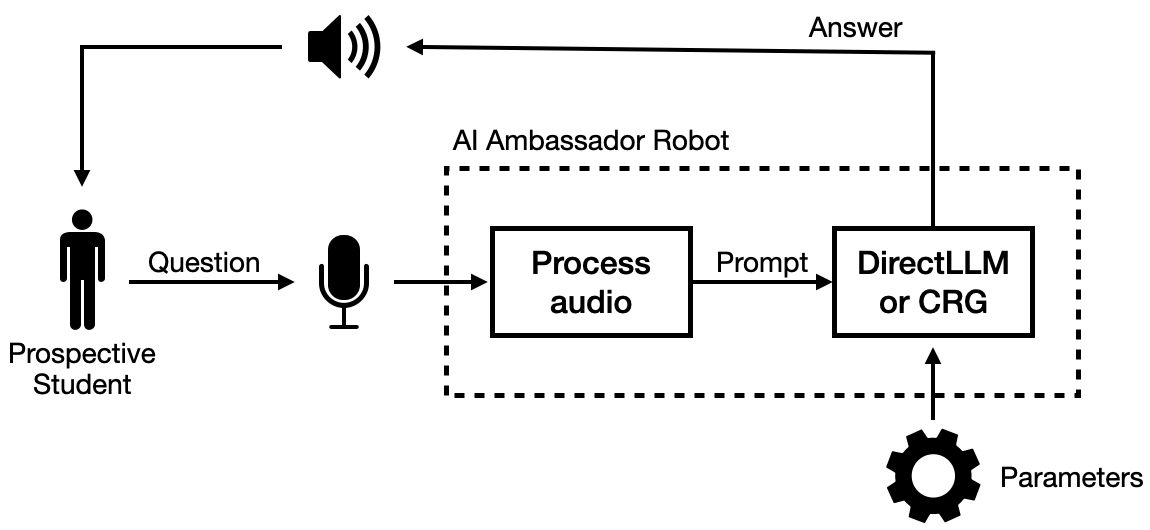
\includegraphics[width=0.70\linewidth]{assets/system_diagram.png}
    \caption{AI Robot System Diagram}
    \label{fig:system}
\end{figure*}

Various mediums to house the underlying AI-powered tour guide were considered. The mediums can be broken up into two categories: kit based systems and custom systems.
The first kit-based system is the MangDang Mini Pupper \cite{b1}, an open-source dog-like robot, powered by a Raspberry Pi 4B. It highlights a simple and quick assembly as well as an all-inclusive kit. 
The second kit-based system is the Poppy Humaniod \cite{b6}, and open-source human-like robot. The Poppy Humaniod is powered by a Raspberry Pi as well, however most of the parts are 3D printed by the customer. The robot utilizes Dynamixel servos to provide stable and accurate movement, the downside being the high cost of the parts.
The last medium considered is a custom system, designed from scratch. This opens up the possibility for the robotic medium to be custom to the department and college. 

Regardless of the robotic medium chosen, the robot will feature three main parts to facilitate an interactive experience: a microphone, a computer, and a speaker. 
A simplified system diagram can be seen in Figure \ref{fig:system}. The prospective student will interact with the robot via the microphone, where their question will be transcribed from audio to text.
This question is then fed into either the DirectLLM pipeline or CRG pipeline. Once the pipeline processes the prompt, it is outputted back to the prospective student via a speaker.

Ultimately, the chosen robotic medium will be the MangDang Mini Pupper. 
The decision was made based on the cost, ease of assembly, and the all-inclusive kit.

%== Custom Dataset Development ==%
\section{Custom Dataset Development}
Due to the niche nature of the application, a custom dataset of question and answer pairs about the LCSEE was developed.
The dataset was created by curating information from various sources, including the LCSEE website, course catalogs, departmental brochures, and talking to tour guides of the department. 
The goal was to ensure that the dataset covered a wide range of topics relevant to prospective students, including academic programs, faculty research, campus facilities, and student life.

Question and answer pairs were human-generated, ensuring accuracy and eliminating the risk of misinformation.
To expand the dataset and improve generalization, data augmentation techniques were employed.
This included paraphrasing questions, rephrasing answers, and introducing synonyms to create variations of the original pairs.
To efficiency augment the dataset, each question answer pair was fed into ChatGPT to generate multiple variations of the same question and answer.

The dataset is stored in the SQuAD format \cite{b7}. 
The SQuAD format includes a list of topics as the top level, with each topic having a title. 
In each topic exist paragraphs, these contain context to the topic and question-answer pairs.
To fit the dataset to the task at hand, the topics were chosen based off of types of questions that could be asked about the department:
degree programs, research opportunities, facilities and resources, clubs and organizations, career opportunities, internships, financial aid and scholarships, faculty information, admission process, and location and contact.

The dataset consists of 421 question-answer pairs, with 10 categories.
A table summarizing the dataset can be seen in Table \ref{tab:dataset}.
\begin{table}[h]
    \centering
    \caption{Custom Dataset Summary}
    \begin{tabular}{|c|c|}
        \hline
        \textbf{Category} & \textbf{Number of Pairs} \\ \hline
        Degree Programs & 55 \\ \hline
        Research Opportunities & 77 \\ \hline
        Facilities and Resources & 85 \\ \hline
        Clubs and Organizations & 71 \\ \hline
        Career Opportunities & 60 \\ \hline
        Internships & 25 \\ \hline
        Financial Aid and Scholarships & 39 \\ \hline
        Faculty Information & 0 \\ \hline
        Admission Process & 0 \\ \hline
        Location and Contact & 9 \\ \hline
    \end{tabular}
    \label{tab:dataset}
\end{table}

% CRG Flow Figure
\begin{figure*}[t]
    \centering
    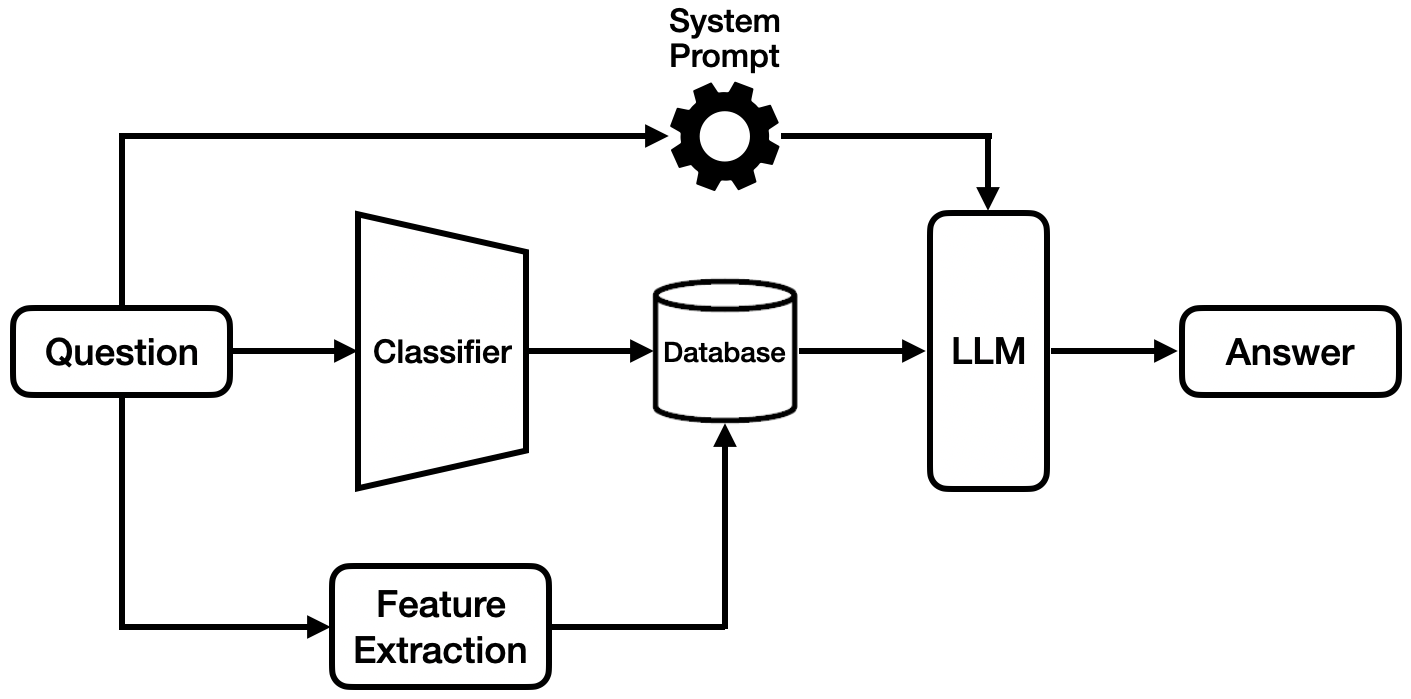
\includegraphics[width=0.60\linewidth]{assets/crg_diagram.png}
    \caption{Classify-Retrieve-Generate (CRG) Pipeline}
    \label{fig:crg_flow}
\end{figure*}

%== DirectLLM Model ==%
\section{DirectLLM Model}
\subsection{Model Selection and Justification}
The DirectLLM model consists of a pre-trained LLM that is fine-tuned on the custom dataset.
To meet the project's objectives, the language model was developed with the following criteria in mind: it had to be open source, capable of effective training on both question-and-answer (Q\&A) datasets and web page content, and optimized for lightweight deployment with quick response times on a microcontroller platform.

An open-source language model was chosen due to their capabilities in lightweight implementations while maintaining high-quality natural language understanding and generation.
Open-source models such as FLAN-T5 \cite{b8} and BART \cite{b9} provide a solid foundation due to their small size and performance on Q\&A task with minimal fine-tuning. 
These models are well-suited for customization and can be fine-tuned with domain-specific data.

Fine-tuned Langauge Agnostic Network (FLAN-T5) is a variant of the T5 (Text-to-Text Transfer Transformer) model, which is pretrained on a diverse range of tasks. 
It features strong ability to be trained on a wide variety of datasets, including Q\&A tasks. 
It also meets the versatile, scalability, and open-source criteria. 
The model used in this project has 77 million parameters, making it lightweight and suitable for deployment on resource-constrained devices.

Bidirectional and Auto-regressive Transformer (BART) is a sequence-to-sequence model optimized for tasks like text generation, summarization, and translation. 
It combines bidirectional context encoding with autoregressive decoding. 
It features capabilities to fine-tune on specific datasets, and effective in both understanding and generating coherent responses.
Like FLAN-T5, it meets the criteria concerned with being open-source, scalable, and versatile. 
The model used in this project has 139 million parameters, making it suitable for deployment on moderately resource-constrained devices.

\subsection{Training and Fine-Tuning Process} 
Both FLAN-T5 and BART were finetuned on the same custom dataset. The model hyperparameters can be found in Table \ref{tab:hyperparams}.
The test dataset included eight questions pertaining to the CSEE department, topics of the questions including: degree programs, research opportunities, student organizations, and career opportunities. 

\begin{table}[!ht]
    \centering
    \caption{Hyperparameters for FLAN-T5 and BART Fine-Tuning}
    \label{tab:hyperparams}
    \begin{tabular}{l|c|c}
        \toprule
        \textbf{Hyperparameter}         & \textbf{FLAN-T5}         & \textbf{BART} \\
        \midrule
        Evaluation Strategy             & Epoch                   & Epoch                     \\ 
        Weight Decay                    & 0.01                    & 0.01                      \\ 
        Learning Rate                   & 5e-5                    & 3e-5                      \\ 
        Logging Steps                   & 5                       & 5                         \\ 
        Train Batch Size                & 8                       & 8                         \\ 
        Evaluation Batch Size           & 8                       & 8                         \\ 
        Number of Training Epochs       & 10                      & 5                         \\ 
        \bottomrule
    \end{tabular}
\end{table}

\subsection{Deployment on Microcontroller}
The implementation of FLAN-T5 and BART leverages Hugging Face Transformers, a comprehensive framework for working with pre-trained language models.
Training was done via the Hugging Face training pipeline, built on the Trainer class and text generation was configured for inference using the Hugging Face pipeline for text generation.
Each model utilized their own transformer: The T5 Tokenizer \cite{b10} for FLAN-T5 and BART Tokenizer \cite{b11} for BART.

% # TODO: deployment on microcontroller 

\subsection{Strengths and Limitations}
% # TODO: strengths and limitations of the model 

%== Classify-Retrieve-Generate (CRG) Model ==%
\section{Classify-Retrieve-Generate (CRG) Model}
To address the issues of how to handle new information in the LCSEE, a new approach is needed. 
Instead of a DirectLLM approach, which would need to be retrained with new information, the classify-retrieve-generate (CRG) approach is proposed. 
The main approach here is to have a neural network classify the question asked into the type of question (i.e. degree programs, research, etc) with some encoded information to look up the answer in a database. 
Once fetched, the raw data is fed into a basic LLM that will refine the response to a more natural response.
The CRG pipeline can be seen in Figure \ref{fig:crg_flow}.

\section{Classification Step}

%== Evaluation and Comparison ==%
\section{Evaluation and Comparison}


%== Discussion ==%
\section{Discussion}


%== Conclusion ==%
\section{Conclusion}


\begin{thebibliography}{00}
\bibitem{b1} Mangdang, "Mangdang Store," Available: https://mangdang.store
\bibitem{b2} M. Rajkomar et al., "Scalable and accurate deep learning with electronic health records," npj Digital Medicine, vol. 1, no. 18, 2018.
\bibitem{b3} T. Dettmers et al., "Sparse fine-tuning for efficient deployment of large-scale language models," NeurIPS Conference Proceedings, 2022.
\bibitem{b4} Z. Jiang et al., "Efficient deep learning inference on edge devices: Challenges and techniques," ACM Computing Surveys, vol. 55, no. 6, 2023.
\bibitem{b5} H. Touvron et al., "Llama 2: Open foundation and fine-tuned chat models," arXiv:2307.09288, 2023.
\bibitem{b6} Poppy Project, "Poppy Humanoid," Available: https://www.poppy-project.org/en/robots/poppy-humanoid/.
\bibitem{b7} R. Rajpurkar, "SQuAD: The Stanford Question Answering Dataset," SQuAD Explorer.
\bibitem{b8} Chung, Hyung Won, Le Hou, Shayne Longpre, Barret Zoph, Yi Tay, William Fedus, Eric Li, et al. "Scaling Instruction-Finetuned Language Models." arXiv (2022). https://doi.org/10.48550/arXiv.2210.11416.
\bibitem{b9} M. Lewis, Y. Liu, N. Goyal, M. Ghazvininejad, A. Mohamed, O. Levy, V. Stoyanov, and L. Zettlemoyer, "BART: Denoising Sequence-to-Sequence Pre-training for Natural Language Generation, Translation, and Comprehension," CoRR, vol. abs/1910.13461, 2019. [Online]. Available: http://arxiv.org/abs/1910.13461.
\bibitem{b10} H. Xu, M. Scales, A. Nguyen, R. Ritter, C. Raffel, K. Shankar, S. A. Saurous, and Q. V. Le, "Deep Evolutionary Reinforcement Learning," arXiv preprint arXiv:1910.10683, 2019. [Online]. Available: https://arxiv.org/pdf/1910.10683.
\bibitem{b11} M. Lewis, Y. Liu, N. Goyal, M. Ghazvininejad, A. Mohamed, O. Levy, V. Stoyanov, and L. Zettlemoyer, "BART: Denoising Sequence-to-Sequence Pre-training for Natural Language Generation, Translation, and Comprehension," arXiv preprint arXiv:1910.13461, 2019. [Online]. Available: https://arxiv.org/pdf/1910.13461. [Accessed: Dec. 17, 2024].
\end{thebibliography}

%-- Appendix --%
\newpage
\onecolumn
\appendix
\section{Appendix}


\end{document}
